% manuscript, to be drafted

%%This is a very basic article template.
%%There is just one section and two subsections.
%\documentclass[12pt,oneside,a4paper,doublespacing]{article} % for submission
\documentclass[11pt,oneside,a4paper]{article} % for sharing

\usepackage{appendix}
\usepackage{amsmath}
\usepackage{caption}
\usepackage{placeins}
\usepackage{graphicx}
\usepackage{subcaption}
%\usepackage{subfig}
\usepackage{longtable}
\usepackage{setspace}
%\usepackage{tikz}
\usepackage{booktabs}
\usepackage{tabularx}
\usepackage{xcolor,colortbl}
\usepackage{chngpage}
%\usepackage[active,tightpage]{preview}
\usepackage{natbib}
\bibpunct{(}{)}{,}{a}{}{;} 
\usepackage{url}
\usepackage{nth}
\usepackage{authblk}
\usepackage[most]{tcolorbox}
%\usepackage{hyperref}
%\usepackage{color}
%\usepackage{fontspec}
%\usepackage{pdfsync}
\usepackage[normalem]{ulem}
\usepackage{amsfonts}
\usepackage{xfrac}
%\renewcommand{\listtablename}{List of Appendix Tables}
%\newcolumntype{C}[1]{>{\centering\let\newline\\\arraybackslash\hspace{0pt}}m{#1}}
%\newcolumntype{L}[1]{>{\raggedright\let\newline\\\arraybackslash\hspace{0pt}}m{#1}}
% working on this need to concatenate file name based on sex and variable name
%\newcommand\Cell[1]{{\raisebox{-0.05in}{\includegraphics[height=.2in,width=.2in]{Figures/ColorCodes/\expandafter#1}}}}  

%%%%%%%%%%%%%%%%%%%%%%%%%%%%%%%%%%%%%%%%%%%%%%%%%%%%%%%%%%%%%%%%%%%%%%%%%%%%%
% setting color to letters affects spacing. Here's a hack I found here:
% http://tex.stackexchange.com/questions/212736/change-letter-colour-without-losing-letter-spacing
%\DeclareRobustCommand{\spacedallcaps}[1]{\MakeUppercase{\textsc{#1}}} % all
% caps with better spacing

%\colorlet{RED}{red}
%\colorlet{BLUE}{b}
%\colorlet{rd}{red}
%\colorlet{bl}{blue}

%%%%%%%%%%%%%%%%%%%%%%%%%%%%%%%%%%%%%%%%%%%%%%%%%%%%%%%%%%%%%%%%%%%%%%%%%%%%%%

\newcommand\ackn[1]{%
  \begingroup
  \renewcommand\thefootnote{}\footnote{#1}%
  \addtocounter{footnote}{-1}%
  \endgroup
}
%\newcommand\vt[1]{\textcolor{rd}{#1}}
%\newcommand\eg[1]{\textcolor{bl}{#1}}

%\newcommand\tg[1]{\includegraphics[scale=.5]{Figures/triadtable/triad#1.pdf}}
%\newcommand\tgh[1]{\raisebox{-.25\height}{\includegraphics[scale=.3]{Figures/triadtable/triad#1.pdf}}}

\defcitealias{HMD}{HMD}
\newcommand{\dd}{\; \mathrm{d}}
\newcommand{\tc}{\quad\quad\text{,}}
\newcommand{\tp}{\quad\quad\text{.}}
% junk for longtable caption
\AtBeginEnvironment{longtable}{\linespread{1}\selectfont}
\setlength{\LTcapwidth}{\linewidth}

%%%%%%%%%%%%%%%%%%%%%%%%%%%%%%%
\begin{document}

\title{Accounting for temporal variation in morbidity measurement
and projections}

\author[1]{Alyson van Raalte\thanks{Authors are currently ordered in reverse
alphabetical order. Correspondence to vanraalte@demogr.mpg.de or
riffe@demogr.mpg.de}}
\author[1]{Tim Riffe}
\affil[1]{Max Planck Institute for Demographic Research}

%\author{[Authors]}

\maketitle

\begin{abstract}
In calculating healthy life expectancy, the use of age-specific morbidity
prevalence data implicitly assumes a chronological age at onset, i.e. that the
disabling process is related to how long an individual has lived. However, many
common disabling processes are better measured by a time-to-death
(thanatological) pattern.
Since death occurs most often at advanced ages, the conflation a mortality
pattern that increases with age and a thanatological morbidity pattern produces
an apparent morbidity pattern that also increases with advancing age. In the
cohort perspective the true and apparent morbidity patterns will imply the same
health expectancies, but problems arise in the period perspective. Comparing the
changes in period health expectancies over time cannot easily be partitioned
into morbidity and mortality components, because the period morbidity component
will depend on some unknown future time-to-death process. In this paper we
illustrate these concepts formally and empirically, using morbidity data from
the Health and Retirement Survey. While holding the time-to-death morbidity
function fixed, we show that mortality reduction alone reduces the total life
years with disability. We estimate the magnitude of this bias for different
disabling processes. This has implications for projections, as well as any
between- or within-population comparisons of period HLE with different age patterns of mortality.
\end{abstract}

\newpage
\section{Introduction}

Healthy life expectancy (HLE) is among the most widely used metrics of population health. It combines information on mortality and morbidity prevalence to summarize the expected years of life lived in good health, however measured. If healthy life expectancy is increasing faster than life expectancy, morbidity is being compressed into a smaller proportion of life. HLE can increase because of changes mortality, morbidity or both. 

In calculating HLE, our use of age-specific morbidity prevalence data implicitly assumes a chronological age at onset, i.e. that the disabling process is related to how long an individual has lived. However, \citet{Riffe2015} have shown that many common disabling processes are better measured by a thanatological (time-to-death) age pattern. Nevertheless, because death occurs most often at advanced ages, the conflation of a chronological mortality pattern and a thanatological morbidity age pattern will produce an apparent morbidity pattern that also increases with advancing age. In the cohort perspective the true and apparent morbidity patterns will be the same. The problems arise in the period perspective. Comparing differences in period HLE between two populations cannot easily be partitioned into morbidity and mortality components, because the period morbidity component will depend on some unknown future time-to-death process. For the same reason, comparisons of disability prevalence rates by age are not recommended between populations with different underlying age schedules of mortality.

 In this paper we illustrate these concepts formally and empirically, using morbidity data from the Health and Retirement Survey. While assuming a fixed time-to-death morbidity function, we show that mortality reduction alone reduces the total life years with disability (DLY). We estimate the magnitude of this bias for different disabling processes, given different levels of mortality. 


\section{Morbidity as a function of thanatological age}
 
Imagine a bad health condition, $G$, that varies as a function of time to death,
$y$, and not as a function of chronological age, $a$. Since the distribution of
times to death is empirically regular, there will still be an apparent age
function, $g^\star(a)$.
In this case $g^\star(a)$ is an aggregate based on both mortality and the real underlying time-to-death process:
 
\begin{align}
g^\star(a) &= \frac{\int _0^\omega g(y) N(a,y) \dd y}{N(a)} \\
      &= \frac{\int _0^\omega g(y) N(a)
      \mu(a+y)\frac{\ell(a+y)}{\ell(a)}\dd y}{N(a)}\\
      &= \int _0^\omega g(y) f(y|a)\dd y \tc
\end{align}
where $N(a)$ is the population aged $a$, $\ell(a)$ is the survival function, and
$\mu(a)$ is the force of mortality. $f(y|a)$ can be interpreted as the
probability of dying in $y$ years given survival to age $a$, and thus the final
expression is purged of population structure. That is, the population of age $a$
that has condition $G$ does not depend on population structure at all, but only
on the force of mortality and the time-to-death pattern of $G$, $g(y)$. 

A function such as $g(y)$ would have implications for the interpretation of
period age patterns of morbidity, and by extension, HLE. If a function such as $g(y)$ holds, it is tautologically true that the
measurement of HLE in completed cohorts (or populations with fixed mortality)
will be identical whether estimated on the basis of $g^\star(a)$ or $g(y)$.
Period HLE is also unproblematic in a fixed mortality setting, as long as future
mortality is also held fixed. Difficulties only arise in the interpretation of
period HLE under changing mortality. For a time-to-death process, forthcoming
improvements in mortality will have the effect of decreasing morbidity today.
This artifact can stymie the projection of today's age patterns of morbidity
into the future: Under changing mortality and a fixed $g(y)$, the age pattern of
morbidity will change even as the morbidity process does not. 

Further, since morbidity is partly a function of mortality, it is difficult to
compare the age patterns of morbidity for populations with different mortality
levels or patterns. Under these circumstance, it is trickier than it seems to
partition differences period HLE into true morbidity and mortality components, because the morbidity component will rely on some unknown future mortality quantity that is a driver of the apparent age pattern of morbidity.
 
We first illustrate this concept with a toy example. 

\begin{figure}
\centering
\begin{subfigure}{.5\textwidth}
  \centering
  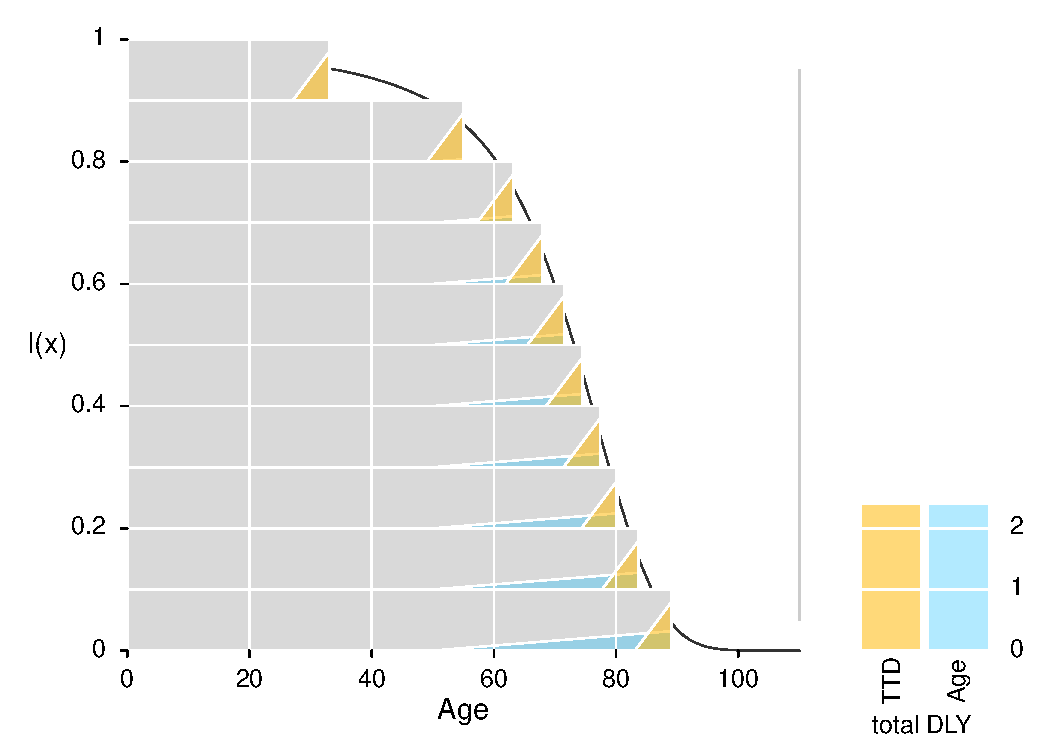
\includegraphics[width=.48\linewidth]{Figures/Japan1970}
  \caption{Higher mortality setting}
  \label{fig:toypop1}
\end{subfigure}%
\begin{subfigure}{.5\textwidth}
  \centering
  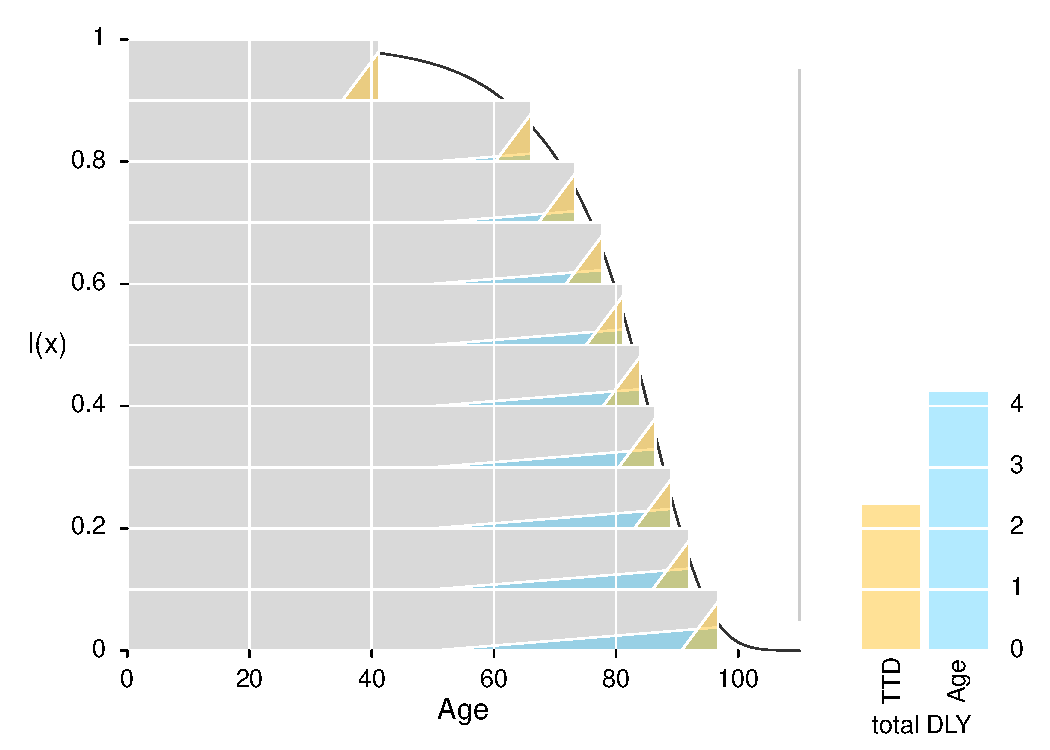
\includegraphics[width=.48\linewidth]{Figures/Japan2010}
  \caption{Lower mortality setting}
  \label{fig:toypop2}
\end{subfigure}
\caption{Schematic chronological (blue) and time-to-death (yellow) morbidity
processes in higher and lower mortality populations.}
\label{fig:test}
\end{figure}
%Assume the population
%process outlined in the Lexis diagram of Figure~\ref{fig:Fig_DiagramLexis}.
% This diagram represents quantities that will induce the aforementioned
% inconsistency.
%Blue numbers on the horizontal age bars represent the number of birthdays,
% while black numbers represent census counts. Red numbers represent deaths in the
%Lexis triangle, and finally, green numbers next to birthdays represent the
%number of unhealthy people that would be alive assuming the pattern of $g(y)$
%found in Figure~\ref{fig:Fig_TTDgy} (given in Appendix Table~\ref{tab:gy}) and
%the given mortality pattern, assuming deaths are distributed uniformly in Lexis
%triangles, and the average values given in Table~\ref{tab:gy} apply. The
% example moves from a higher mortality stationary setting to a lower mortality stationary
%setting.
%
%\begin{figure}
%\begin{adjustwidth}{-1.5cm}{}
%	\centering
%	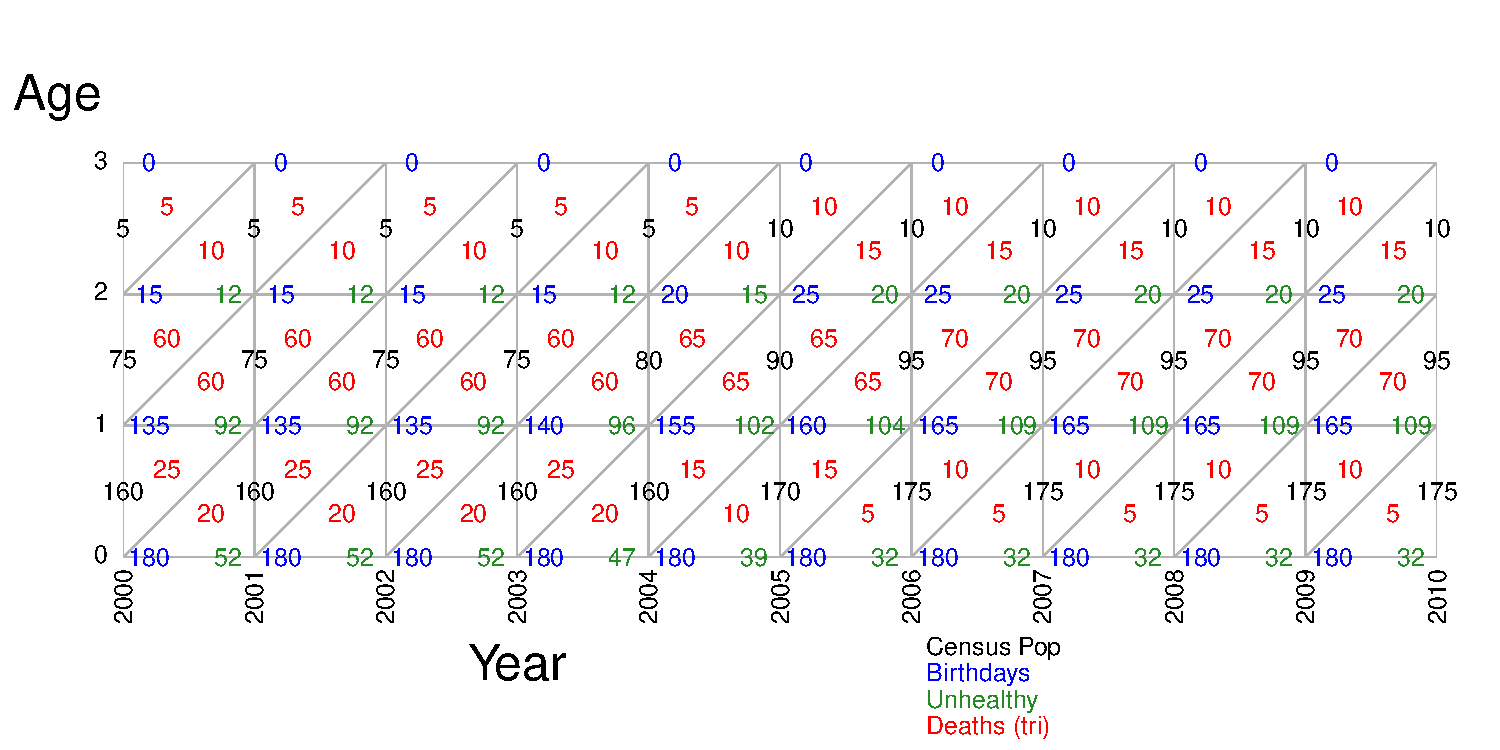
\includegraphics[scale=.6]{DiagramLexis.pdf}
%	\caption{The Lexis diagram}
%	\label{fig:Fig_DiagramLexis}
%\end{adjustwidth}
%\end{figure}
%
%
%
%\begin{figure}
%\begin{adjustwidth}{-1.5cm}{}
%	\centering
%	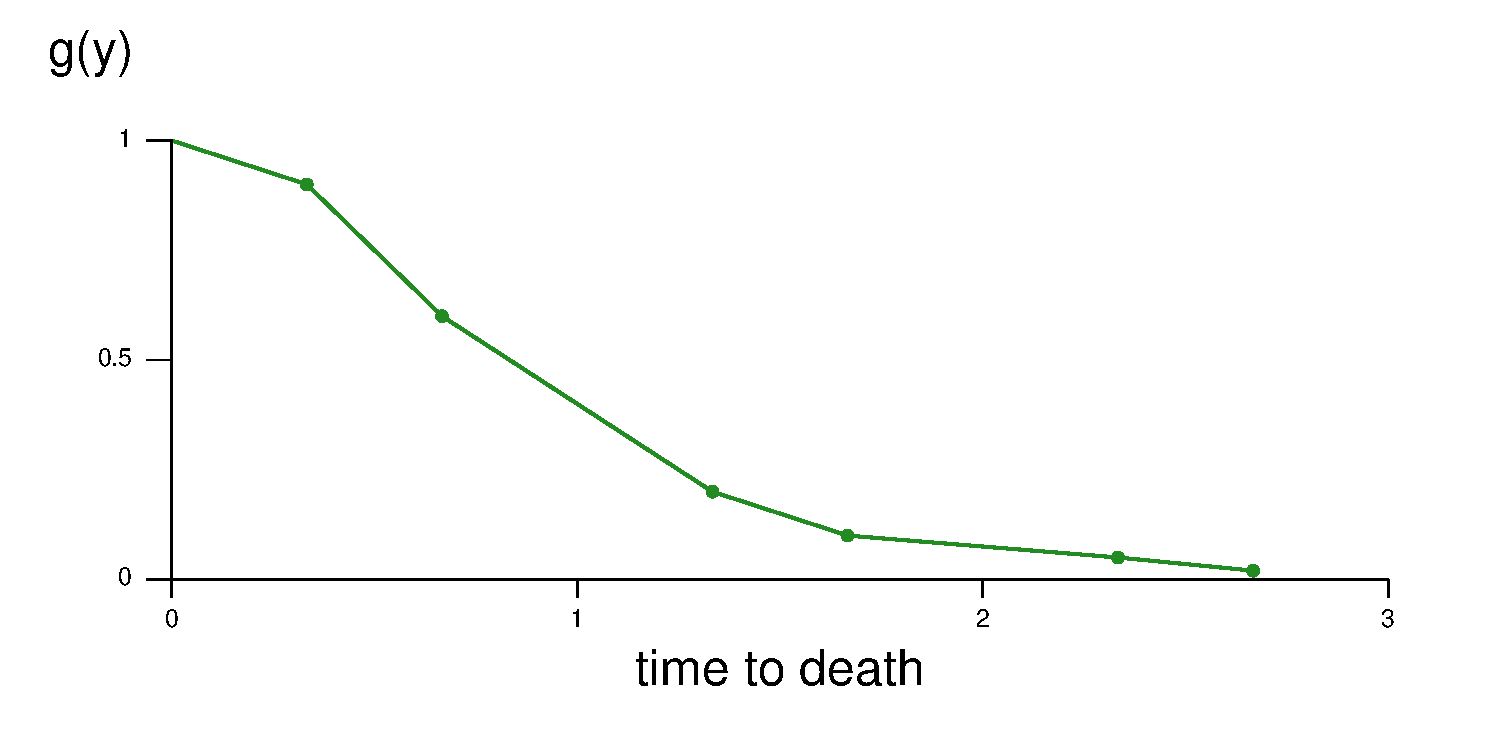
\includegraphics[scale=.6]{TTDgy.pdf}
%	\caption{The time-to-death profile of disability of the toy example}
%	\label{fig:Fig_TTDgy}
%\end{adjustwidth}
%\end{figure}
%
%To calculate the numbers unhealthy in any given birthday line, first note that
%the average years lived in a Lexis triangle by those dying in the triangle is
%$\sfrac{1}{3}$. For example, 20 of the
%babies born in the year 2003 will die within the year. These deaths have an
%average lifespan of $\sfrac{1}{3}$, and so they contribute $20\times0.90$
%% unhealthy people to the birth cohort at age 0 (value from appendix
% table~\ref{tab:gy}.
%Those dying from the same cohort before age 1 in the year 2004 contribute
%$15\times0.6$ unhealthy persons to age 0 in 2003, and so forth iteratively up
%the cohort.
%
%In this controlled setting, where the underlying $g(y)$ is held fixed, we can
%calculate both the period and cohort HLE values.\footnote{See Appendix
%explanations for the details used to calculate lifetables and mean values of
%$G(a)$. } Figure~\ref{fig:e0eHtoy} shows trends in period and cohort total and
%healthy life expectancy. In the initial and final stages, period and cohort
%healthy and total life expectancies agree, because these are the stationary
%start and end of the series. As is usually the case, there is no perfect way to
%compare cohort and period line graphs, since the x-axis refers to both cohort
%and period. 

%\begin{figure}
%\begin{adjustwidth}{-1.5cm}{}
%	\centering
%	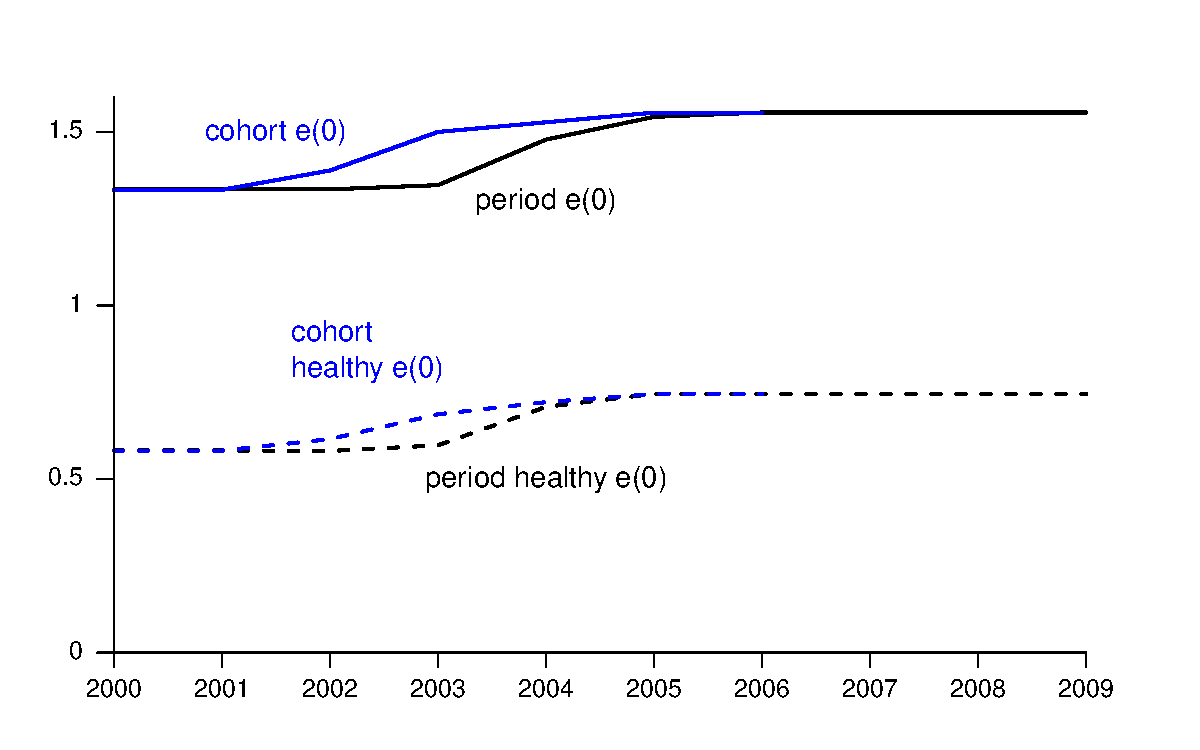
\includegraphics[scale=.6]{e0eHtoy.pdf}
%	\caption{Cohort and period life expectancy and healthy life expectancy.}
%	\label{fig:e0eHtoy}
%\end{adjustwidth}
%\end{figure}
%
%The gap between year 2001 and 2005 marks an inconsistency. In
%this case, the inconsistency is entirely driven by mortality change. Further
% the gap in HLE is due not only to the change in the survival function used to
%calculate HLE, but also to changes in the pattern of $g^\star(a)$. That is,
%if we were to decompose the difference in 2001 and 2007 HLE using conventional
%methods, there would appear to be a morbidity contribution to the difference,
%even though morbidity in this case is held fixed. We demonstrate such an
%inconsistency using somewhat more realistic data in the following section.
% 
%


\section{Sex differences in Healthy Life Expectancy}

Let's again assume that morbidity is a thanatological age function. Using empirically observed US data we can initiate changing sex differences in age-specific morbidity prevalence and healthy life expectancy, arising solely from period mortality decline.

Morbidity data come from the US Health and Retirement Study, specifically difficulties in carrying out functional Activities of Daily Living. The disability prevalence was calculated by the average number of difficulties in ADL experienced at each age for the 1915 birth cohort divided by the total ADLs. Because the cohort was nearly extinct, we were able to calculate both the thanatological $g(y)$ and chronological $g(a)$ age profiles of disability prevalence, borrowing information from neighbouring cohorts to obtain smooth age profiles using a Loess filter. 

The resulting ADL-disability prevalence is illustrated in Figure \ref{fig:ADL_thana-chrono}. The horizontally running gradients indicate that time-to-death is the more important time axis to predict deterioration in ADL than time since birth. Thus our assumption of a thanatological age function of morbidity is not unrealistic. This is the case for many, but not all, indicators of health \citep{Riffe2015}. At our oldest observed age, 6 percent of males and 11 percent of females were still alive. Both morbidity and mortality rates were forecasted to close the cohort out at age 110.  Mortality and exposure data came from the Human Mortality Database \citep{HMD2015}. 

Next we calculated the apparent age function of morbidity $g^\star(a)$ that would have occurred in 1995 and 2010, had the individuals been subject to the 1915 cohort $g(y)$ (Figure \ref{fig:morb_age}). For simplicity we assumed that the 1995 and 2010 period life tables came from stationary populations. Thus any changes to the 1995 and 2010 $g^\star(a)$ schedules resulted exclusively from observed mortality change between the periods, and not by the underlying morbidity function. For both men and women, the disability prevalence declined below age 100. Had we observed these patterns, we would have artificially congratulated ourselves on reducing or postponing the disabling process, when in fact all we did was to reduce mortality. That males showed greater declines in age-specific disability prevalence was strictly owing to their stronger mortality decline than females.

Although the changes in disability prevalence induced by mortality decline are not large, they do result in absolute increases in expected years of life in a state of disability at age 74 (Table \ref{tab:HLE_HRS}). If we were to decompose temporal differences in healthy life expectancy, at each age we would have non-zero components that are conventionally thought of as mortality and morbidity effects even though we have not changed the underlying morbidity function. 

\begin{table}[ht]
	\centering
		\begin{tabular}{l|rrrr}
			\toprule
		 \quad & \textbf{Females} & \quad & \textbf{Males} & \quad  \\	
		 \quad & \textbf{1995} & \textbf{2010} & \textbf{1995} & \textbf{2010} \\
	\midrule
	Expected Healthy Life Years&10.3&11.2&8.7&10.3\\
	Expected Disabled Life Years&2.5&2.5&1.4&1.5\\
	Expected Total Life Years&12.7&13.8&10.1&11.8\\
	Proportion of Life healthy&0.81&0.82&0.86&0.88\\

	\bottomrule		
		\end{tabular}
	\caption{HLE at age 74 and its components under changing period mortality but morbidity fixed to the observed 1915 cohort g(y)}
	\label{tab:HLE_HRS}
\end{table}




\begin{figure}
	\centering
		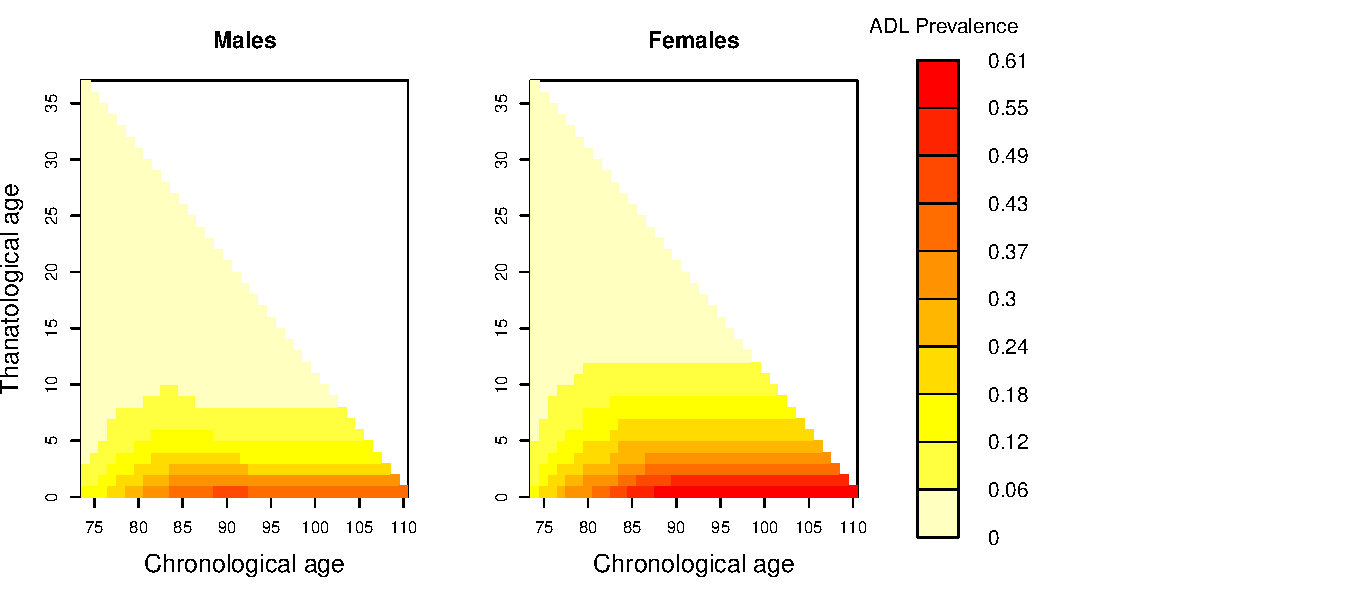
\includegraphics[width=1.1\textwidth]{Fig_ADL_thana-chrono_rev.pdf}
	\caption{The prevalence of ADL impairment as a function of both thanatological and chronological age}
	\label{fig:ADL_thana-chrono}
\end{figure}




\begin{figure}
	\centering
		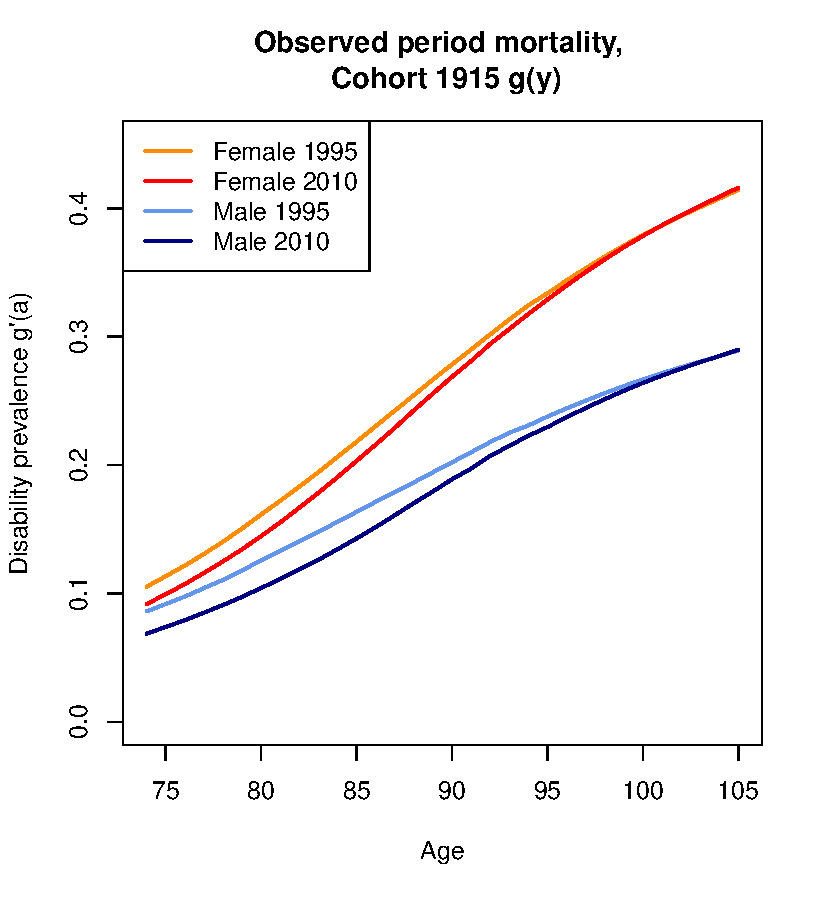
\includegraphics[width=0.7\textwidth]{morb_by_age_1915gy.pdf}
	\caption{The changing age-specific disability prevalence induced by mortality change alone}
	\label{fig:morb_age}
\end{figure}



\section{Future considerations}
The results using the US HRS data at this point are meant to be illustrative, but robustness checks are still needed. Specifically, we will check the robustness of our smoothing technique of the ADL prevalence surface and our mortality forecasts for the 6 and 11 percent of the cohort still alive in the most recent survey. Using established decomposition techniques \citep{Andreev2002,Horiuchi2008}, we will further explore the implications of mortality and morbidity perturbations on sex differences in healthy life expectancy. 
Finally, the paper as it stands now is mostly theoretical. By PAA we hope to further develop the empirical components. Specifically, we aim to see whether we can explain some of the observed sex differences in HLE by accounting for different thanatological vs chronological patterning of morbidity.


\section{Discussion}




Healthy life expectancy remains a popular tool for analyzing population health. At any given time, a snapshot of the life years lived in good or poor health are captured. This information is accurately summarized in both the period and cohort perspective, regardless of whether morbidity is a function of chronological or thanatological age. The difficulties arise in the interpretation of period differences in this quantity. The chronological age pattern of disability can increase or decrease solely as a function of mortality change even when the underlying morbidity function is held constant. Thus, for instance, observed widening ratios in the age profiles of disability prevalence between subgroups \citep{Crimmins2001} cannot be attributed to changes in the disabling process without taking into account changing mortality profiles. This also calls into question the practice of forecasting observed age-specific rates of decline in disability \citep{Manton2006,Khaw1999}. Health economists refer to a similar 'red herring' argument, namely that medical costs are more closely associated with time-to-death than with chronological age. As a result, health care cost projections based on a chronological rather than thanatological age pattern of mortality are artificially inflated \citep{Zweifel1999,Geue2014}.

Instead, we argue that the better way to measure changes in health or disability is from a cohort perspective \citep{Manton2000,Manton2008,Christensen2013}. \citet{Manton2000}, for instance, found large differences between period and cohort estimates of active life expectancy (ALE). ALE at ages 65 and 85 was between 1.6 and 2.6 times larger in the cohort perspective than for similar period estimates, and the expected years of life disabled were smaller. Additionally, they uncovered larger differences between the cohort and period perspectives for men than women, which they attribute to differences in disability transition rates between the sexes. We theorize that some of these larger differences might also be attributable to larger mortality reduction among men.

Several studies have looked at the macro relationship between overall mortality levels and sex differences in HLE. At higher levels of life expectancy, female advantage in healthy life expectancy diminishes, or even reverses into male advantage \citep{vanOyen2013}. Meanwhile, the larger the proportional female advantage in longevity, the larger the female excess in the proportion of life in poor health \citep{Luy2014}. That mortality levels and disability prevalence are related is perhaps not surprising. As our example illustrates, differences in the underlying mortality lead to differences in the age profile of disability. Additionally, although the association between the severity of chronic conditions and poor health was found to be similar for men and women, morbidity prevalence rates are generally higher among women, particularly for arthritis and chronic pain \citep{Case2005}. It would be worthwhile to investigate whether there might not only be differences in the composition of chronic conditions between the sexes, but whether the underlying morbidity process itself might differ between the sexes in its chronological versus thanatological axis \citep{Riffe2015}. 

In reality, not all end-of-life health conditions are exclusive functions of
time-to-death, but morbidity often varies as a function of
both chronological and thanatological age, and it is best to express morbidity
as a function of both age and time-to-death, $g(a,y)$. There is great variety in
the temporal variation of late-life health conditions \citep{Riffe2015}.
Further, the function $g(a,y)$ changes over time and it is not fixed as in our examples. Nevertheless, the distortions demonstrated are likely to arise in everyday practice when comparing health trends over age between populations
and over time, since many health conditions appear to show strong time-to-death
components. Trends in mortality may offset or amplify changes in morbidity.
Therefore, in order to separate effects, more careful measurements are required
than is typically the case. 

\section{Appendix}

Given the numbers from Figure~\ref{fig:Fig_DiagramLexis}, there are various methods that one can use to
calculate period and cohort lifetables. For the sake of reproducibility for our
toy example, we describe steps as follows, first for periods, then for cohorts.
\subsection{Period quantities}
We use event exposure lifetables, though it would be possible to jump straight
to death quotients from the given Lexis diagram.
Exposures for age $x$ in year $t$, $E(x,t)$, are calculated, per the HMD Methods
Protocol \citep{Wilmoth2007} as:
\begin{equation}
E(x,t) = \frac{C(x,t) + C(x,t+1)}{2} + \frac{D_L(x,t) - D_U(x,t)}{6} \tc
\end{equation}
where $C(x,t)$ is the census population in age interval $[x,x+1)]$ on January 1
of year $t$, $D_L(x,t)$ are deaths in the lower Lexis triangle of age $x$ in
year $t$, i.e., belonging to the cohort born in the year interval $[t-x,t-x+1)$.
$D_U(x,t)$ are deaths in the upper Lexis triangle of age $x$ in
year $t$, i.e., belonging to the cohort born in the year interval
$[t-x-1,t-x)$. All standard period lifetable steps are followed from the HMD
Methods Protocol, with the exception of the $a(x)$ assumption. The HMD assumes period $a(x)$
values of $\frac{1}{2}$. Instead, we apply the following formula:
\begin{equation}
a(x,t) = \frac{D_L(x,t)\frac{1}{3} + D_U(x,t)\frac{2}{3}}{D_L(x,t) + D_U(x,t)}
\tp
\end{equation}
We then proceed to calculate all columns through $e(x)$. 

The average value of the unhealthy condition $G$ at age $x$in year $t$, $g(x,t)$
is calculated as follows. We first convert counts unhealthy on birthdays to
proportions, and then take the arithmetic average of the proportion unhealthy at
age $x$ and age $x+1$. Expectancies are then calculated as follows:
\begin{align}
e(0,t) =&\sum _0^2 L(x,t) \\
e_U(0,t) =&\sum _0^2 L(x,t) g(x,t) \\
e_H(0,t) =& e(0,t) - e_U(0,t) \tc
\end{align}
where $e(0,t)$ is the life expectancy at birth in year $t$, $e_U(0,t)$ is
unhealthy life expectancy, and $e_H(0,t)$ is healthy life expectancy.

\subsection{Cohort quantities}
For cohorts we proceed directly from within-cohort age interval survival
probabilities, $p(x,c)$, as follows:
\begin{equation}
p(x,c) = \frac{B(x+1,c)}{B(x,c)} \tc
\end{equation}
where $B$ are birthdays (horizontal counts), $x$ indexes the lower age interval
bound, and $c$ is the cohort born in the year interval $[c,c+1)]$. Starting with
a radix of 1, we calculate $l(x,c)$ as:
\begin{equation}
l(x,c) = \prod_0^x p(a,c)
\end{equation}
$L(x,c)$ is calculated as the arithmetic average of lower $l(x,c)$ and
$l(x+1,c)$. The average value of $G$ for the AC parallelogram is calculated
similarly as for period squares, except that we take the arithmetic average of
the proportions unhealthy at birthday $x$ and $x+a$ within the same cohort.
Expectancies are then calculated in the same way.

\subsection{Values assumed for $g(y)$ in toy example}
If deaths in Lexis triangles are distributed uniformly, then the average year
lived of those dying in the triangle is $\sfrac{1}{3}$. Since deaths in the
example Lexis diagram are given in triangles, we assume values of $g(y)$ for the
average years lived for the deaths in each triangle. For example, 20 of the
babies born in the year 2003 will die within the year, and these have an average
lifespan of $\sfrac{1}{3}$, and so they contribute $20\times0.90$ unhealthy
people to the birth cohort at age 0. 

 \begin{table}[ht]
\centering
\begin{tabular}{rr}
\hline
TTD & $g(y)$ \\
\hline
$\sfrac{1}{3}$ & 0.90 \\
$\sfrac{2}{3}$ & 0.60 \\
$1\sfrac{1}{3}$ & 0.20 \\
$1\sfrac{2}{3}$ & 0.10 \\
$2\sfrac{1}{3}$ & 0.05 \\
$2\sfrac{2}{3}$ & 0.02 \\
\hline
\end{tabular}
\caption{$g(y)$ used in toy example.}
\label{tab:gy}
\end{table}



\newpage%% this forces a new page, so that things end up a bit more where you think they should
\bibliographystyle{chicago}
\bibliography{refs}

\end{document}
